\section{Taxonomy}
\label{sec:taxonomy}

\begin{figure}[t]
  \centering
  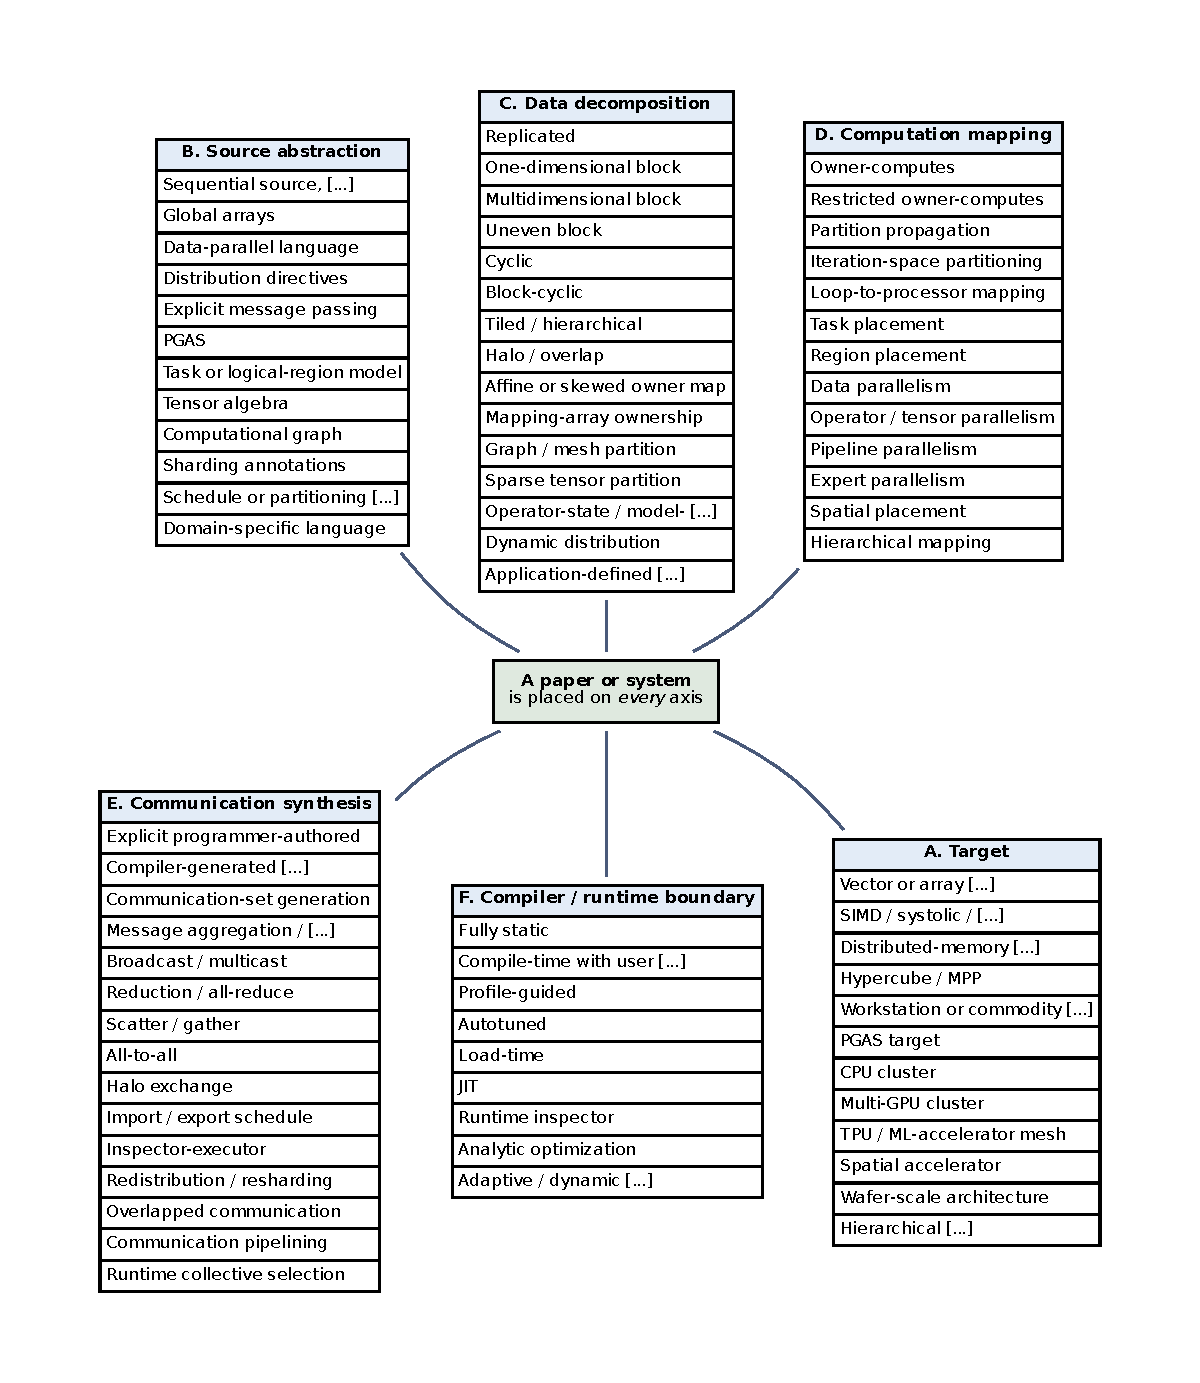
\includegraphics[width=\columnwidth]{taxonomy.pdf}
  \caption{The taxonomy is a set of orthogonal axes, not a tree: each paper or system takes one or more values on every axis. Only the six axes used most in the text are shown; the catalog carries eleven. Generated from the machine-readable taxonomy so that the figure cannot drift from the catalog.}
  \label{fig:taxonomy}
\end{figure}

\ours{We classify each paper or system along eleven independent axes (Fig.~\ref{fig:taxonomy}): (A)~target and memory model; (B)~programming abstraction (RQ1); (C)~data decomposition (RQ2); (D)~computation mapping (RQ3); (E)~communication synthesis (RQ4); (F)~compilation time, i.e. the compiler/runtime boundary (RQ5); (G)~compiler architecture; (H)~optimization objective (RQ7); (I)~maturity and artifact status; (J)~paper type; and (K)~compiler representation (RQ6).} The value lists are maintained in the repository and enforced by a validator.

\subsection{Why chronology alone is insufficient}
\infer{HPF (1993) and GSPMD (2021) take the same values on axis~C (block distribution over a logical processor grid) and on axis~E (communication inserted by propagating distributions through the program), yet they are three eras apart; inspector--executor runtimes (1990) and distributed sparse-tensor compilers (2022--2025) share the \emph{runtime inspector} value on axis~F.} A chronological list hides these recurrences, which are among the survey's main findings (Section~\ref{sec:synthesis}). Chronology is therefore one dimension (Section~\ref{sec:history}), used to explain \emph{why} a value was chosen at a given time, while the axes explain \emph{what} was chosen.

\subsection{Provenance of category names}
Where a standard term exists we use it: \emph{owner-computes} from the Kali/Fortran~D literature, \emph{inspector--executor} from PARTI, \emph{BLOCK}, \emph{CYCLIC}, and \emph{block-cyclic} from HPF, \emph{partition propagation} from GSPMD, \emph{inter-} and \emph{intra-operator parallelism} from Alpa~\cite{zheng2022alpa}. The grouping of these into axes, and the decision to place ML sharding compilers and wafer-scale compilers on the same axes as 1990s HPF compilers, is ours.

\subsection{Tagging discipline}
A tag is attached to a catalog entry only when an evidence pointer names the section of the primary source supporting it. Entries whose full text has not been consulted are tagged only on the axes their abstract clearly supports. Lineage fields record only relationships that a paper states itself or that a cited survey states; inferred lineages are kept separately. Table~\ref{tab:eras} summarises the eras, Table~\ref{tab:systems} the core systems, and Tables~\ref{tab:decomposition}--\ref{tab:evaluation} the decomposition support, compiler architecture, and evaluation methodology of each system; all are generated from the catalog.

% AUTO-GENERATED by scripts/generate_tables.py from catalog/*.yaml -- do not edit by hand.

\begin{table*}[t]
\centering
\scriptsize
\caption{Era summary. Dates are provisional (see Sec.~\ref{sec:methodology}); representative systems are the catalog entries with the highest reading priority in each era.}
\label{tab:eras}
\begin{tabular}{p{0.11\textwidth}p{0.12\textwidth}p{0.14\textwidth}p{0.14\textwidth}p{0.14\textwidth}p{0.10\textwidth}p{0.15\textwidth}}
\toprule
\textbf{Era} & \textbf{Machine driver} & \textbf{Programming abstraction} & \textbf{Decomposition representation} & \textbf{Generated communication} & \textbf{Representative systems} & \textbf{Limitation} \\
\midrule
0: Foundations (1950--1979) & Stored-program machines, FORTRAN, pipelined vector processors, lock-step array processors, dataflow and systolic proposals & Sequential FORTRAN; vector statements; early parallel-language proposals & None for distribution; dependence graphs and loop-level analysis for vectorization & None (shared or centralised memory) & -- & No notion of data placement as a compiler problem; machines had a single address space or SIMD broadcast control \\
1: Emergence of distributed-memory compilation (1980--1987) & Multicomputers and hypercubes (Cosmic Cube, iPSC, nCUBE), systolic arrays, Connection Machine & Explicit message passing; early global-array proposals; SIMD data-parallel languages & Programmer-managed; first compiler proposals for placement & Hand-written sends/receives & -- & Programming by hand was error-prone; portability across machines was poor \\
2: Global arrays and data decomposition (1988--1992) & Commercial hypercubes and MPPs (iPSC/2, iPSC/860, nCUBE-2, CM-2) & Sequential or global-array programs with distribution annotations (SUPERB, Kali, Vienna Fortran, Fortran D) & BLOCK/CYCLIC distributions, alignment to templates/decompositions, overlap regions & Compiler-generated point-to-point messages; message vectorization; first inspector-executor runtimes & \cite{callahan1988compiling,koelbel1991compiling,hiranandani1992compiling,li1991alignment} & Regular, affine programs only; automatic distribution selection intractable in general; communication costs poorly modelled \\
3: HPF, MPI, and compiler maturity (1993--2000) & MPPs (CM-5, Paragon, SP2, T3D/T3E) and early clusters & HPF directives; MPI library calls; irregular extensions; early PGAS proposals (Co-array Fortran, Titanium) at the end of the era & HPF ALIGN/DISTRIBUTE with BLOCK, CYCLIC(k), templates and processor arrangements; INDIRECT/mapping arrays in HPF-2 and research systems & Communication sets, local address generation, redistribution, collectives; PARTI/CHAOS schedules for irregular code & \cite{zima1993compiling,benkner1999compiling,banerjee1995paradigm,loveman1993hpf} & HPF compilers were slow to mature and performance was unpredictable; explicit MPI became the dominant practice \\
4: MPI dominance and alternative programming models (2000--2010) & Commodity clusters, early multicore nodes, Cell/BE and explicitly managed memories & MPI(+OpenMP); PGAS (UPC, Co-array Fortran, Titanium); HPCS languages (Chapel, X10); hierarchical memory models (Sequoia) & Language-level distributions and locales/places; hierarchical task trees & One-sided communication, compiler-scheduled bulk transfers for memory hierarchies & \cite{tang2000tiled,chen2003upc,charles2005x10,diaconescu2005reusable} & Adoption of new languages remained limited; automatic distribution rarely used in production \\
5: Compiler/runtime co-design and accelerators (2010--2019) & GPU clusters, heterogeneous nodes, early TPU pods & Affine loop nests; task/region programs (Legion, Regent); tensor DSLs; ML graph frameworks & Polyhedral partitions; logical regions and partitions; named-dimension layouts (Mesh-TensorFlow) & Polyhedral communication-set generation with MPI; dynamic region coherence; collectives in ML frameworks & \cite{bondhugula2013compiling,kruse2014molly,bondhugula2011automatic,bauer2012legion} & Each system covered one domain; no shared ownership IR; ML partitioning still largely manual \\
6: Mesh sharding, ML systems, and spatial accelerators (2020--2026) & TPU/GPU pods, AI accelerators, wafer-scale engines, spatial dataflow chips & Sharding annotations on device meshes; tensor algebra with distribution formats; MLIR dialects; stencil DSLs & Device meshes with per-dimension sharding; distributed tensor formats; MLIR shard/mesh attributes & Collective insertion by propagation; resharding; automated search over parallelism plans & \cite{xu2021gspmd,zheng2022alpa,alabed2025partir,yadav2022distal} & Dynamic/irregular workloads, heterogeneous hierarchies, and memory-capacity constraints remain weakly handled; fragmentation across frameworks \\
\bottomrule
\end{tabular}
\end{table*}

% AUTO-GENERATED by scripts/generate_tables.py from catalog/*.yaml -- do not edit by hand.

\begin{table*}[t]
\centering
\scriptsize
\caption{Core systems in the catalog. A question mark marks a cell not yet verified from a primary source.}
\label{tab:systems}
\begin{tabular}{p{0.08\textwidth}p{0.05\textwidth}p{0.06\textwidth}p{0.11\textwidth}p{0.12\textwidth}p{0.11\textwidth}p{0.12\textwidth}p{0.09\textwidth}p{0.10\textwidth}p{0.08\textwidth}}
\toprule
\textbf{System} & \textbf{Refs} & \textbf{Years} & \textbf{Input} & \textbf{Distribution} & \textbf{Work mapping} & \textbf{Communication} & \textbf{Runtime} & \textbf{Targets} & \textbf{Artifact} \\
\midrule
SUPERB & \cite{zima1988superb,gerndt1990updating} & 1986-1992 & Fortran 77 + interactive distribution & ? & ? & ? & SUPRENUM MP & SUPRENUM & unavailable \\
Kali & \cite{mehrotra1990kali,koelbel1991compiling} & 1989-1992 & Fortran + dist + doall/on & block, cyclic, block\_cyclic, user map, dynamic & on clause / owner() & in/out sets static or run-time inspector & cached inspector/executor & iPSC-class multicomputers & unavailable \\
PARTI / CHAOS & \cite{saltz1990runtime,saltz1991multiprocessor} & 1989-1997 & irregular loops with index arrays & mapping arrays via translation tables; partitioner-driven & iteration partitioning via RIG/partitioner & inspector-built import/export schedules; schedule reuse & PARTI/CHAOS & iPSC/2, iPSC/860, CM-2 & unavailable \\
Fortran D & \cite{callahan1988compiling,hiranandani1991fortrand} & 1991-1996 & Fortran 77 + decomposition directives & ? & ? & ? & NX / PARTI & iPSC/860 & unavailable \\
Vienna Fortran / VFCS & \cite{chapman1991vienna,chapman1992vienna} & 1991-1999 & Fortran 77 + DIST/ALIGN & block, cyclic(k), user-defined, INDIRECT, dynamic & owner computes; FORALL ON & overlap areas, vectorised messages (VFCS) & VFCS & iPSC/860, GENESIS, SUPRENUM & unavailable \\
PARADIGM & \cite{gupta1992automatic,su1993paradigm} & 1992-1997 & Fortran 77 (automatic) & ? & ? & ? & ? & iPSC, Paragon, CM-5 (to verify) & unavailable \\
Fortran 90D/HPF (Syracuse) & \cite{bozkus1993fortran90d} & 1993-1995 & Fortran 90D & ? & ? & runtime collective library & F90D runtime & ? & unavailable \\
High Performance Fortran (language) & \cite{loveman1993hpf,hpfforum1993spec} & 1993-2000 & Fortran 90 + directives & BLOCK, CYCLIC, CYCLIC(k), replicated; 2.0 adds INDIRECT, GEN\_BLOCK & implementation-defined (owner computes typical) & implementation-defined & n/a & n/a & specification \\
Digital (DEC) Fortran 90 HPF compiler & \cite{harris1995dechpf} & 1994-1998 & HPF 1.1 & BLOCK, CYCLIC, replicated, alignment & data-parallel; owner computes not strictly enforced & region assignments; vectorised sends; shadow edges; inlined reductions & PSE SEND/RECEIVE & Alpha workstation farms, AlphaServer SMP & commercial, unavailable \\
Titanium & \cite{yelick1998titanium} & 1998-2010 & Titanium (Java dialect) & ? & SPMD & ? & GASNet & clusters & archived \\
Co-array Fortran & \cite{numrich1998coarray} & 1998-present & Fortran + [ ] co-dimensions & one co-array per image & SPMD, programmer & explicit co-array references & ? & Cray T3E and later & spec; Fortran 2008 coarrays \\
Unified Parallel C (Berkeley UPC) & \cite{chen2003upc} & 2002-present & UPC & ? & upc\_forall affinity & ? & GASNet & clusters & open source \\
X10 & \cite{charles2005x10} & 2004-2020 & X10 & ? & at(place) / async & ? & X10RT & clusters & archived \\
Chapel & \cite{chamberlain2007chapel} & 2005-present & Chapel & user-defined domain maps (Block, Cyclic, BlockCyclic, Replicated, ...) & forall over distributed domains; on clauses & compiler + runtime (GET/PUT, aggregation) & Chapel runtime & clusters, GPUs & open source \\
Sequoia & \cite{fatahalian2006sequoia} & 2006-2010 & task trees & ? & task-to-memory-level mapping & bulk copies between levels & Sequoia runtime & Cell, clusters & unavailable \\
Pluto distributed-memory code generation (Bondhugula et al.) & \cite{bondhugula2008pluto,bondhugula2011automatic} & 2011-2016 & C affine loop nests & derived from computation partition (flow-out sets) & polyhedral iteration-space partitioning & polyhedral communication sets to MPI & MPI / dynamic scheduler & InfiniBand clusters & open source (pluto distmem branch) \\
Legion / Regent & \cite{bauer2012legion,slaughter2015regent} & 2012-present & tasks + logical regions & region partitions chosen by program/mapper & mapper interface & runtime-managed coherence and copies & Legion/Realm & GPU clusters & open source \\
Molly & \cite{kruse2014molly} & 2014-2015 & C++ + layout declarations & programmer-declared & polyhedral & generated asynchronous MPI & MPI & Blue Gene/Q (intended) & archived \\
Mesh-TensorFlow & \cite{shazeer2018meshtf} & 2018-2021 & TF graph + named dims + layout & dimension-to-mesh-axis layout & SPMD per layout & allreduce/allgather/alltoall derived from layouts & TF/TPU & TPUv2 pods & archived \\
FlexFlow & \cite{jia2019flexflow} & 2018-present & operator graph & SOAP output-tensor partitions & MCMC search with simulator & task graph with transfer tasks & FlexFlow/Legion & P100/K80 clusters & open source \\
XLA SPMD partitioner (GShard / GSPMD) & \cite{lepikhin2020gshard,xu2021gspmd} & 2020-present & HLO + sharding annotations & replicated / tiled / partially tiled per tensor over device mesh & SPMD; sharding propagation & collectives + halo exchange + resharding inserted per operator & XLA & TPUv3 pods (GPU supported) & open source (XLA) \\
Cerebras WSE programming (CSL / hand-mapped stencils) & \cite{rocki2020cerebras,jacquelin2022wse} & 2020-present & CSL & programmer-placed per-PE tiles & spatial placement & fabric colours / routes configured by programmer & SDK & CS-1/CS-2/CS-3 & commercial SDK \\
PartIR & \cite{alabed2025partir} & 2021-2025 & StableHLO + tactics & ? & ? & ? & XLA & TPU, GPU & ? \\
DISTAL / SpDISTAL & \cite{yadav2022distal,yadav2022spdistal} & 2022-2023 & tensor index notation + formats + schedule & tensor distribution notation over a processor grid; sparse non-zero/universe partitions & distribute/communicate/rotate schedule to index-task launches & Legion partitions (bounds analysis; image/preimage for sparse) & Legion & Lassen CPU/GPU nodes & open source \\
Alpa & \cite{zheng2022alpa} & 2022-2023 & JAX graph & per-stage sharding specs (ILP) & DP over stages/submeshes + ILP intra-op & GSPMD collectives + cross-mesh resharding & Alpa MPMD runtime & 64x V100 & archived \\
MLIR shard dialect (formerly mesh) & \cite{mlir2025shard} & 2023-present & MLIR + shard.grid/shard.sharding & per-axis grid sharding with halos & SPMD & all\_gather, all\_reduce, all\_to\_all, reduce\_scatter, update\_halo, send/recv & n/a & n/a & upstream MLIR \\
xDSL stencil / dmp / mpi stack & \cite{bisbas2024shared,stawinoga2026mlir} & 2023-present & stencil DSLs & static Cartesian rank-grid decomposition (dmp) & owner computes per block; one z-column per PE on WSE & dmp.swap halo exchange to mpi dialect or CSL chunked prefetch & MPI / CSL library & ARCHER2, GPUs, FPGA, CS-2/CS-3 & open source \\
Shardy (OpenXLA) & \cite{openxla2024shardy} & 2024-present & StableHLO + SDY shardings & per-axis mesh shardings & propagation & ? & XLA & TPU, GPU & open source \\
\bottomrule
\end{tabular}
\end{table*}

% AUTO-GENERATED by scripts/generate_tables.py from catalog/*.yaml -- do not edit by hand.

\begin{table}[t]
\centering
\scriptsize
\caption{Decomposition support by system. $\bullet$ supported, $\circ\!\!\bullet$ partial, $\circ$ not supported, ? not yet verified.}
\label{tab:decomposition}
\begin{tabular}{lcccccccc}
\toprule
\textbf{System} & \textbf{block} & \textbf{cyclic} & \textbf{block-cyclic} & \textbf{replication} & \textbf{halo} & \textbf{dynamic} & \textbf{irregular} & \textbf{hierarchical} \\
\midrule
SUPERB & ? & ? & ? & ? & $\textbackslash\{\}bullet$ & ? & ? & $\textbackslash\{\}circ$ \\
Kali & $\textbackslash\{\}bullet$ & $\textbackslash\{\}bullet$ & $\textbackslash\{\}bullet$ & $\textbackslash\{\}bullet$ & ? & $\textbackslash\{\}bullet$ & $\textbackslash\{\}circ\textbackslash\{\}!\textbackslash\{\}!\textbackslash\{\}bullet$ & $\textbackslash\{\}circ$ \\
PARTI / CHAOS & $\textbackslash\{\}bullet$ & $\textbackslash\{\}circ$ & $\textbackslash\{\}circ$ & $\textbackslash\{\}circ$ & $\textbackslash\{\}circ$ & $\textbackslash\{\}bullet$ & $\textbackslash\{\}bullet$ & $\textbackslash\{\}circ$ \\
Fortran D & ? & ? & ? & ? & ? & ? & ? & $\textbackslash\{\}circ$ \\
Vienna Fortran / VFCS & $\textbackslash\{\}bullet$ & $\textbackslash\{\}bullet$ & $\textbackslash\{\}bullet$ & $\textbackslash\{\}bullet$ & $\textbackslash\{\}bullet$ & $\textbackslash\{\}circ\textbackslash\{\}!\textbackslash\{\}!\textbackslash\{\}bullet$ & $\textbackslash\{\}bullet$ & $\textbackslash\{\}circ$ \\
PARADIGM & ? & ? & ? & ? & ? & $\textbackslash\{\}bullet$ & ? & $\textbackslash\{\}circ$ \\
Fortran 90D/HPF (Syracuse) & ? & ? & ? & ? & ? & ? & ? & $\textbackslash\{\}circ$ \\
High Performance Fortran (language) & $\textbackslash\{\}bullet$ & $\textbackslash\{\}bullet$ & $\textbackslash\{\}bullet$ & $\textbackslash\{\}bullet$ & $\textbackslash\{\}circ$ & $\textbackslash\{\}bullet$ & $\textbackslash\{\}circ\textbackslash\{\}!\textbackslash\{\}!\textbackslash\{\}bullet$ & $\textbackslash\{\}circ$ \\
Digital (DEC) Fortran 90 HPF compiler & $\textbackslash\{\}bullet$ & $\textbackslash\{\}bullet$ & ? & $\textbackslash\{\}bullet$ & $\textbackslash\{\}bullet$ & $\textbackslash\{\}circ$ & $\textbackslash\{\}circ\textbackslash\{\}!\textbackslash\{\}!\textbackslash\{\}bullet$ & $\textbackslash\{\}circ$ \\
Titanium & ? & ? & ? & ? & ? & ? & ? & ? \\
Co-array Fortran & $\textbackslash\{\}bullet$ & $\textbackslash\{\}circ$ & $\textbackslash\{\}circ$ & $\textbackslash\{\}bullet$ & $\textbackslash\{\}circ$ & $\textbackslash\{\}circ$ & $\textbackslash\{\}circ$ & $\textbackslash\{\}circ$ \\
Unified Parallel C (Berkeley UPC) & $\textbackslash\{\}bullet$ & $\textbackslash\{\}bullet$ & $\textbackslash\{\}bullet$ & $\textbackslash\{\}circ$ & $\textbackslash\{\}circ$ & $\textbackslash\{\}circ$ & $\textbackslash\{\}circ$ & $\textbackslash\{\}circ$ \\
X10 & ? & ? & ? & ? & ? & ? & ? & ? \\
Chapel & $\textbackslash\{\}bullet$ & $\textbackslash\{\}bullet$ & $\textbackslash\{\}bullet$ & $\textbackslash\{\}bullet$ & $\textbackslash\{\}circ\textbackslash\{\}!\textbackslash\{\}!\textbackslash\{\}bullet$ & $\textbackslash\{\}circ\textbackslash\{\}!\textbackslash\{\}!\textbackslash\{\}bullet$ & $\textbackslash\{\}circ\textbackslash\{\}!\textbackslash\{\}!\textbackslash\{\}bullet$ & $\textbackslash\{\}circ\textbackslash\{\}!\textbackslash\{\}!\textbackslash\{\}bullet$ \\
Sequoia & ? & ? & ? & ? & ? & ? & ? & $\textbackslash\{\}bullet$ \\
Pluto distributed-memory code generation (Bondhugula et al.) & $\textbackslash\{\}bullet$ & ? & ? & ? & ? & $\textbackslash\{\}circ$ & $\textbackslash\{\}circ$ & $\textbackslash\{\}circ\textbackslash\{\}!\textbackslash\{\}!\textbackslash\{\}bullet$ \\
Legion / Regent & $\textbackslash\{\}bullet$ & $\textbackslash\{\}circ\textbackslash\{\}!\textbackslash\{\}!\textbackslash\{\}bullet$ & $\textbackslash\{\}circ\textbackslash\{\}!\textbackslash\{\}!\textbackslash\{\}bullet$ & $\textbackslash\{\}bullet$ & $\textbackslash\{\}bullet$ & $\textbackslash\{\}bullet$ & $\textbackslash\{\}bullet$ & $\textbackslash\{\}bullet$ \\
Molly & $\textbackslash\{\}bullet$ & ? & ? & ? & ? & $\textbackslash\{\}circ$ & $\textbackslash\{\}circ$ & ? \\
Mesh-TensorFlow & $\textbackslash\{\}bullet$ & $\textbackslash\{\}circ$ & $\textbackslash\{\}circ$ & $\textbackslash\{\}bullet$ & $\textbackslash\{\}circ$ & $\textbackslash\{\}circ$ & $\textbackslash\{\}circ$ & $\textbackslash\{\}circ$ \\
FlexFlow & $\textbackslash\{\}bullet$ & $\textbackslash\{\}circ$ & $\textbackslash\{\}circ$ & $\textbackslash\{\}bullet$ & $\textbackslash\{\}circ$ & $\textbackslash\{\}circ$ & $\textbackslash\{\}circ$ & $\textbackslash\{\}circ$ \\
XLA SPMD partitioner (GShard / GSPMD) & $\textbackslash\{\}bullet$ & $\textbackslash\{\}circ$ & $\textbackslash\{\}circ$ & $\textbackslash\{\}bullet$ & $\textbackslash\{\}bullet$ & $\textbackslash\{\}circ$ & $\textbackslash\{\}circ$ & $\textbackslash\{\}bullet$ \\
Cerebras WSE programming (CSL / hand-mapped stencils) & $\textbackslash\{\}bullet$ & $\textbackslash\{\}circ$ & $\textbackslash\{\}circ$ & $\textbackslash\{\}circ$ & $\textbackslash\{\}bullet$ & $\textbackslash\{\}circ$ & $\textbackslash\{\}circ\textbackslash\{\}!\textbackslash\{\}!\textbackslash\{\}bullet$ & $\textbackslash\{\}circ$ \\
PartIR & ? & ? & ? & ? & ? & ? & ? & ? \\
DISTAL / SpDISTAL & $\textbackslash\{\}bullet$ & $\textbackslash\{\}circ$ & $\textbackslash\{\}circ$ & $\textbackslash\{\}bullet$ & $\textbackslash\{\}circ$ & $\textbackslash\{\}circ\textbackslash\{\}!\textbackslash\{\}!\textbackslash\{\}bullet$ & $\textbackslash\{\}bullet$ & $\textbackslash\{\}bullet$ \\
Alpa & $\textbackslash\{\}bullet$ & $\textbackslash\{\}circ$ & $\textbackslash\{\}circ$ & $\textbackslash\{\}bullet$ & $\textbackslash\{\}circ$ & $\textbackslash\{\}circ$ & $\textbackslash\{\}circ$ & $\textbackslash\{\}bullet$ \\
MLIR shard dialect (formerly mesh) & $\textbackslash\{\}bullet$ & $\textbackslash\{\}circ$ & $\textbackslash\{\}circ$ & $\textbackslash\{\}bullet$ & $\textbackslash\{\}bullet$ & $\textbackslash\{\}circ$ & $\textbackslash\{\}circ$ & $\textbackslash\{\}circ\textbackslash\{\}!\textbackslash\{\}!\textbackslash\{\}bullet$ \\
xDSL stencil / dmp / mpi stack & $\textbackslash\{\}bullet$ & $\textbackslash\{\}circ$ & $\textbackslash\{\}circ$ & $\textbackslash\{\}circ$ & $\textbackslash\{\}bullet$ & $\textbackslash\{\}circ$ & $\textbackslash\{\}circ$ & $\textbackslash\{\}circ$ \\
Shardy (OpenXLA) & $\textbackslash\{\}bullet$ & ? & ? & $\textbackslash\{\}bullet$ & ? & ? & $\textbackslash\{\}circ$ & ? \\
\bottomrule
\end{tabular}
\end{table}

% AUTO-GENERATED by scripts/generate_tables.py from catalog/*.yaml -- do not edit by hand.

\begin{table}[t]
\centering
\scriptsize
\caption{Compiler architecture by system (from catalog tags).}
\label{tab:architecture}
\begin{tabular}{lccccccp{0.3\columnwidth}}
\toprule
\textbf{System} & \textbf{src-to-src} & \textbf{polyhedral} & \textbf{graph IR} & \textbf{multi-level IR} & \textbf{MLIR} & \textbf{runtime co-design} & \textbf{Generated target} \\
\midrule
SUPERB & $\textbackslash\{\}bullet$ & $\textbackslash\{\}circ$ & $\textbackslash\{\}circ$ & $\textbackslash\{\}circ$ & $\textbackslash\{\}circ$ & $\textbackslash\{\}circ$ & Distributed-memory multicomputer \\
Kali & $\textbackslash\{\}bullet$ & $\textbackslash\{\}circ$ & $\textbackslash\{\}circ$ & $\textbackslash\{\}circ$ & $\textbackslash\{\}circ$ & $\textbackslash\{\}bullet$ & Distributed-memory multicomputer, Hypercube / MPP \\
PARTI / CHAOS & $\textbackslash\{\}circ$ & $\textbackslash\{\}circ$ & $\textbackslash\{\}circ$ & $\textbackslash\{\}circ$ & $\textbackslash\{\}circ$ & $\textbackslash\{\}bullet$ & Hypercube / MPP, Distributed-memory multicomputer \\
Fortran D & $\textbackslash\{\}bullet$ & $\textbackslash\{\}circ$ & $\textbackslash\{\}circ$ & $\textbackslash\{\}circ$ & $\textbackslash\{\}circ$ & $\textbackslash\{\}circ$ & Hypercube / MPP \\
Vienna Fortran / VFCS & $\textbackslash\{\}bullet$ & $\textbackslash\{\}circ$ & $\textbackslash\{\}circ$ & $\textbackslash\{\}circ$ & $\textbackslash\{\}circ$ & $\textbackslash\{\}circ$ & Distributed-memory multicomputer, Hypercube / MPP \\
PARADIGM & $\textbackslash\{\}bullet$ & $\textbackslash\{\}circ$ & $\textbackslash\{\}circ$ & $\textbackslash\{\}circ$ & $\textbackslash\{\}circ$ & $\textbackslash\{\}circ$ & Hypercube / MPP \\
Fortran 90D/HPF (Syracuse) & $\textbackslash\{\}bullet$ & $\textbackslash\{\}circ$ & $\textbackslash\{\}circ$ & $\textbackslash\{\}circ$ & $\textbackslash\{\}circ$ & $\textbackslash\{\}circ$ & Hypercube / MPP \\
High Performance Fortran (language) & $\textbackslash\{\}circ$ & $\textbackslash\{\}circ$ & $\textbackslash\{\}circ$ & $\textbackslash\{\}circ$ & $\textbackslash\{\}circ$ & $\textbackslash\{\}circ$ & Distributed-memory multicomputer \\
Digital (DEC) Fortran 90 HPF compiler & $\textbackslash\{\}circ$ & $\textbackslash\{\}circ$ & $\textbackslash\{\}circ$ & $\textbackslash\{\}circ$ & $\textbackslash\{\}circ$ & $\textbackslash\{\}bullet$ & Workstation or commodity cluster \\
Titanium & $\textbackslash\{\}bullet$ & $\textbackslash\{\}circ$ & $\textbackslash\{\}circ$ & $\textbackslash\{\}circ$ & $\textbackslash\{\}circ$ & $\textbackslash\{\}circ$ & PGAS target \\
Co-array Fortran & $\textbackslash\{\}circ$ & $\textbackslash\{\}circ$ & $\textbackslash\{\}circ$ & $\textbackslash\{\}circ$ & $\textbackslash\{\}circ$ & $\textbackslash\{\}circ$ & PGAS target \\
Unified Parallel C (Berkeley UPC) & $\textbackslash\{\}bullet$ & $\textbackslash\{\}circ$ & $\textbackslash\{\}circ$ & $\textbackslash\{\}circ$ & $\textbackslash\{\}circ$ & $\textbackslash\{\}circ$ & PGAS target \\
X10 & $\textbackslash\{\}bullet$ & $\textbackslash\{\}circ$ & $\textbackslash\{\}circ$ & $\textbackslash\{\}circ$ & $\textbackslash\{\}circ$ & $\textbackslash\{\}circ$ & PGAS target \\
Chapel & $\textbackslash\{\}bullet$ & $\textbackslash\{\}circ$ & $\textbackslash\{\}circ$ & $\textbackslash\{\}circ$ & $\textbackslash\{\}circ$ & $\textbackslash\{\}circ$ & PGAS target, CPU cluster, Multi-GPU cluster \\
Sequoia & $\textbackslash\{\}circ$ & $\textbackslash\{\}circ$ & $\textbackslash\{\}circ$ & $\textbackslash\{\}circ$ & $\textbackslash\{\}circ$ & $\textbackslash\{\}bullet$ & Hierarchical heterogeneous system, CPU cluster \\
Pluto distributed-memory code generation (Bondhugula et al.) & $\textbackslash\{\}bullet$ & $\textbackslash\{\}bullet$ & $\textbackslash\{\}circ$ & $\textbackslash\{\}circ$ & $\textbackslash\{\}circ$ & $\textbackslash\{\}circ$ & CPU cluster, Multi-GPU cluster \\
Legion / Regent & $\textbackslash\{\}circ$ & $\textbackslash\{\}circ$ & $\textbackslash\{\}circ$ & $\textbackslash\{\}circ$ & $\textbackslash\{\}circ$ & $\textbackslash\{\}bullet$ & Multi-GPU cluster, Hierarchical heterogeneous system, CPU cluster \\
Molly & $\textbackslash\{\}circ$ & $\textbackslash\{\}bullet$ & $\textbackslash\{\}circ$ & $\textbackslash\{\}circ$ & $\textbackslash\{\}circ$ & $\textbackslash\{\}circ$ & CPU cluster \\
Mesh-TensorFlow & $\textbackslash\{\}circ$ & $\textbackslash\{\}circ$ & $\textbackslash\{\}bullet$ & $\textbackslash\{\}circ$ & $\textbackslash\{\}circ$ & $\textbackslash\{\}circ$ & TPU / ML-accelerator mesh \\
FlexFlow & $\textbackslash\{\}circ$ & $\textbackslash\{\}circ$ & $\textbackslash\{\}bullet$ & $\textbackslash\{\}circ$ & $\textbackslash\{\}circ$ & $\textbackslash\{\}circ$ & Multi-GPU cluster \\
XLA SPMD partitioner (GShard / GSPMD) & $\textbackslash\{\}circ$ & $\textbackslash\{\}circ$ & $\textbackslash\{\}bullet$ & $\textbackslash\{\}circ$ & $\textbackslash\{\}circ$ & $\textbackslash\{\}circ$ & TPU / ML-accelerator mesh, Multi-GPU cluster \\
Cerebras WSE programming (CSL / hand-mapped stencils) & $\textbackslash\{\}circ$ & $\textbackslash\{\}circ$ & $\textbackslash\{\}circ$ & $\textbackslash\{\}circ$ & $\textbackslash\{\}circ$ & $\textbackslash\{\}circ$ & Wafer-scale architecture \\
PartIR & $\textbackslash\{\}circ$ & $\textbackslash\{\}circ$ & $\textbackslash\{\}circ$ & $\textbackslash\{\}circ$ & $\textbackslash\{\}bullet$ & $\textbackslash\{\}circ$ & TPU / ML-accelerator mesh, Multi-GPU cluster \\
DISTAL / SpDISTAL & $\textbackslash\{\}circ$ & $\textbackslash\{\}circ$ & $\textbackslash\{\}circ$ & $\textbackslash\{\}circ$ & $\textbackslash\{\}circ$ & $\textbackslash\{\}bullet$ & Multi-GPU cluster, CPU cluster \\
Alpa & $\textbackslash\{\}circ$ & $\textbackslash\{\}circ$ & $\textbackslash\{\}bullet$ & $\textbackslash\{\}circ$ & $\textbackslash\{\}circ$ & $\textbackslash\{\}circ$ & Multi-GPU cluster \\
MLIR shard dialect (formerly mesh) & $\textbackslash\{\}circ$ & $\textbackslash\{\}circ$ & $\textbackslash\{\}circ$ & $\textbackslash\{\}circ$ & $\textbackslash\{\}bullet$ & $\textbackslash\{\}circ$ & TPU / ML-accelerator mesh, Multi-GPU cluster, CPU cluster \\
xDSL stencil / dmp / mpi stack & $\textbackslash\{\}circ$ & $\textbackslash\{\}circ$ & $\textbackslash\{\}circ$ & $\textbackslash\{\}bullet$ & $\textbackslash\{\}bullet$ & $\textbackslash\{\}circ$ & CPU cluster, Multi-GPU cluster, Wafer-scale architecture \\
Shardy (OpenXLA) & $\textbackslash\{\}circ$ & $\textbackslash\{\}circ$ & $\textbackslash\{\}circ$ & $\textbackslash\{\}circ$ & $\textbackslash\{\}bullet$ & $\textbackslash\{\}circ$ & TPU / ML-accelerator mesh, Multi-GPU cluster \\
\bottomrule
\end{tabular}
\end{table}

% AUTO-GENERATED by scripts/generate_tables.py from catalog/*.yaml -- do not edit by hand.

\begin{table*}[t]
\centering
\scriptsize
\caption{Evaluation methodology by system. A question mark marks a cell not yet extracted from the primary source.}
\label{tab:evaluation}
\begin{tabular}{p{0.14\textwidth}p{0.14\textwidth}p{0.14\textwidth}p{0.14\textwidth}p{0.14\textwidth}p{0.14\textwidth}p{0.14\textwidth}}
\toprule
\textbf{System} & \textbf{Benchmarks} & \textbf{Baseline} & \textbf{Scale} & \textbf{Metrics} & \textbf{Productivity eval.} & \textbf{Artifact} \\
\midrule
SUPERB & ? & ? & ? & ? & ? & unavailable \\
Kali & ? & ? & ? & ? & ? & unavailable \\
PARTI / CHAOS & ? & ? & ? & ? & ? & unavailable \\
Fortran D & ? & ? & ? & ? & ? & unavailable \\
Vienna Fortran / VFCS & ? & ? & ? & ? & ? & unavailable \\
PARADIGM & ? & ? & ? & ? & ? & unavailable \\
Fortran 90D/HPF (Syracuse) & ? & ? & ? & ? & ? & unavailable \\
High Performance Fortran (language) & ? & ? & ? & ? & ? & specification \\
Digital (DEC) Fortran 90 HPF compiler & ? & ? & ? & ? & ? & commercial, unavailable \\
Titanium & ? & ? & ? & ? & ? & archived \\
Co-array Fortran & ? & ? & ? & ? & ? & spec; Fortran 2008 coarrays \\
Unified Parallel C (Berkeley UPC) & ? & ? & ? & ? & ? & open source \\
X10 & ? & ? & ? & ? & ? & archived \\
Chapel & ? & ? & ? & ? & ? & open source \\
Sequoia & ? & ? & ? & ? & ? & unavailable \\
Pluto distributed-memory code generation (Bondhugula et al.) & ? & ? & ? & ? & ? & open source (pluto distmem branch) \\
Legion / Regent & ? & ? & ? & ? & ? & open source \\
Molly & ? & ? & ? & ? & ? & archived \\
Mesh-TensorFlow & ? & ? & ? & ? & ? & archived \\
FlexFlow & ? & ? & ? & ? & ? & open source \\
XLA SPMD partitioner (GShard / GSPMD) & ? & ? & ? & ? & ? & open source (XLA) \\
Cerebras WSE programming (CSL / hand-mapped stencils) & ? & ? & ? & ? & ? & commercial SDK \\
PartIR & ? & ? & ? & ? & ? & ? \\
DISTAL / SpDISTAL & ? & ? & ? & ? & ? & open source \\
Alpa & ? & ? & ? & ? & ? & archived \\
MLIR shard dialect (formerly mesh) & ? & ? & ? & ? & ? & upstream MLIR \\
xDSL stencil / dmp / mpi stack & ? & ? & ? & ? & ? & open source \\
Shardy (OpenXLA) & ? & ? & ? & ? & ? & open source \\
\bottomrule
\end{tabular}
\end{table*}

